%!TEX program = xelatex 
\documentclass{standalone}%opcao draft remove os links
\usepackage{amssymb,amsmath,amsfonts,amsthm,amstext,pxfonts}
\usepackage{graphicx}
\usepackage[usenames,dvipsnames]{xcolor}
\usepackage{subfigure}
\usepackage{tikz,tikz-3dplot,tkz-euclide,circuitikz,siunitx,pstricks-add,pst-coil,pst-3dplot}
\usepackage{pst-plot,pst-func,pst-eucl,pst-solides3d}
\usetkzobj{all}
\usetikzlibrary{scopes}
\usetikzlibrary{through}
\usetikzlibrary{lindenmayersystems}
\usetikzlibrary[shadings]
\usetikzlibrary{arrows}
\usetikzlibrary{intersections,positioning}

\newcommand{\norm}[1]{\left\Vert{#1}\right\Vert}
\newcommand{\eq}{=}

\begin{document}
    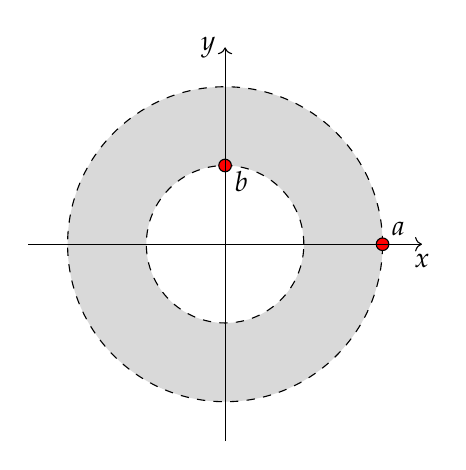
\begin{tikzpicture}
        \coordinate (F) at (-2.5,0);
        \coordinate (G) at (0,-2.5);
        \coordinate (X) at (2.5,0);
        \coordinate (Y) at (0,2.5);
        \coordinate[label=right:$a$] (A) at (2,0.2);
        \coordinate[label=right:$b$] (B) at (0,0.8);
        % Styles
        \tikzstyle{axes}=[]

        \draw[fill=gray!30,even odd rule,style=dashed] (0,0) circle (2cm) circle (1cm) ;
        \draw[fill=red] (0,1) circle (0.08cm);
        \draw[fill=red] (2,0) circle (0.08cm);
        \begin{scope}[style=axes]%constr\'oi os eixos cartesianos
          \draw[->] (F) -- (X) node[below] {$x$} coordinate(x axis);
          \draw[->] (G) -- (Y) node[left] {$y$} coordinate(y axis);
        \end{scope}
    \end{tikzpicture}
\end{document}